\subsection{Ransac with baseline}
Ransac is a procedure which can be used to detect outlying data. We will use Ransac to sort out the correspondences we have found which are too imprecise to contribute to the estimation of the fundamental matrix. Using Ransac makes our estimation of the fundamental matrix more robust, and so we will also look at how robust our estimation becomes by adding random correspondences and then attempt to remove false correspondences with Ransac.

\subsubsection{Problems with Ransac}
Ransac can be implemented in a few different ways. One could simply use the largest inlier set found and return this. One could also estimate the error, and although a bigger inlier set might be found, it will only be accepted if the error is smaller than the previous best set (the set with the smallest error and largest number of inliers). Then, should the points used to compute the model be included when computing this error, or only points not used in the model estimation? In the latter we avoid bias, but the points used for model estimation will most likely be quantified as inliers. And perhaps most importantly, how does one estimate the thresholding use to determine inliers from outliers?\\
After some experimentation I have found using the largest inlier set gave the most consistent results and have thus chosen to use this implementation. For thresholding a constant threshold of 20 have been used. As the threshold is often simply chosen empirically, and the scanline agreement error from the baseline shows decent results, a threshold of 20 seems reasonable. The threshold could also have been estimated based on the standard deviation and a Chi distribution. To determine whether a correspondence is within this threshold, the \textit{Sampson distance} have been used as this seems to the most natural way to estimate the error, and it only involves the fundamental matrix.

\subsubsection{Error as function of falsely added correspondences}
We will now take a look at how robust the fundamental matrix estimation is when using Ransac. For this we take our 25 manually found correspondences and add a number of false correspondence before running Ransac. We then measure the mean and standard deviation of the scanline agreement error. As Ransac is a non-deterministic algorithm we might get rather different errors each run, and because we only are interested in the tendency of how the error behaves when adding false correspondences, we make 10 runs of Ransac and report the median mean and standard deviation found. This helps us avoid lucky or unlucky runs where the error reported is 'uncharacteristic' for the number of false correspondences added, and to avoid the skewness the average would give if one run reports something completely different than the other runs. The results can be seen in \autoref{BaselineRansacMedian}.

\begin{figure}[h]
	\centering
	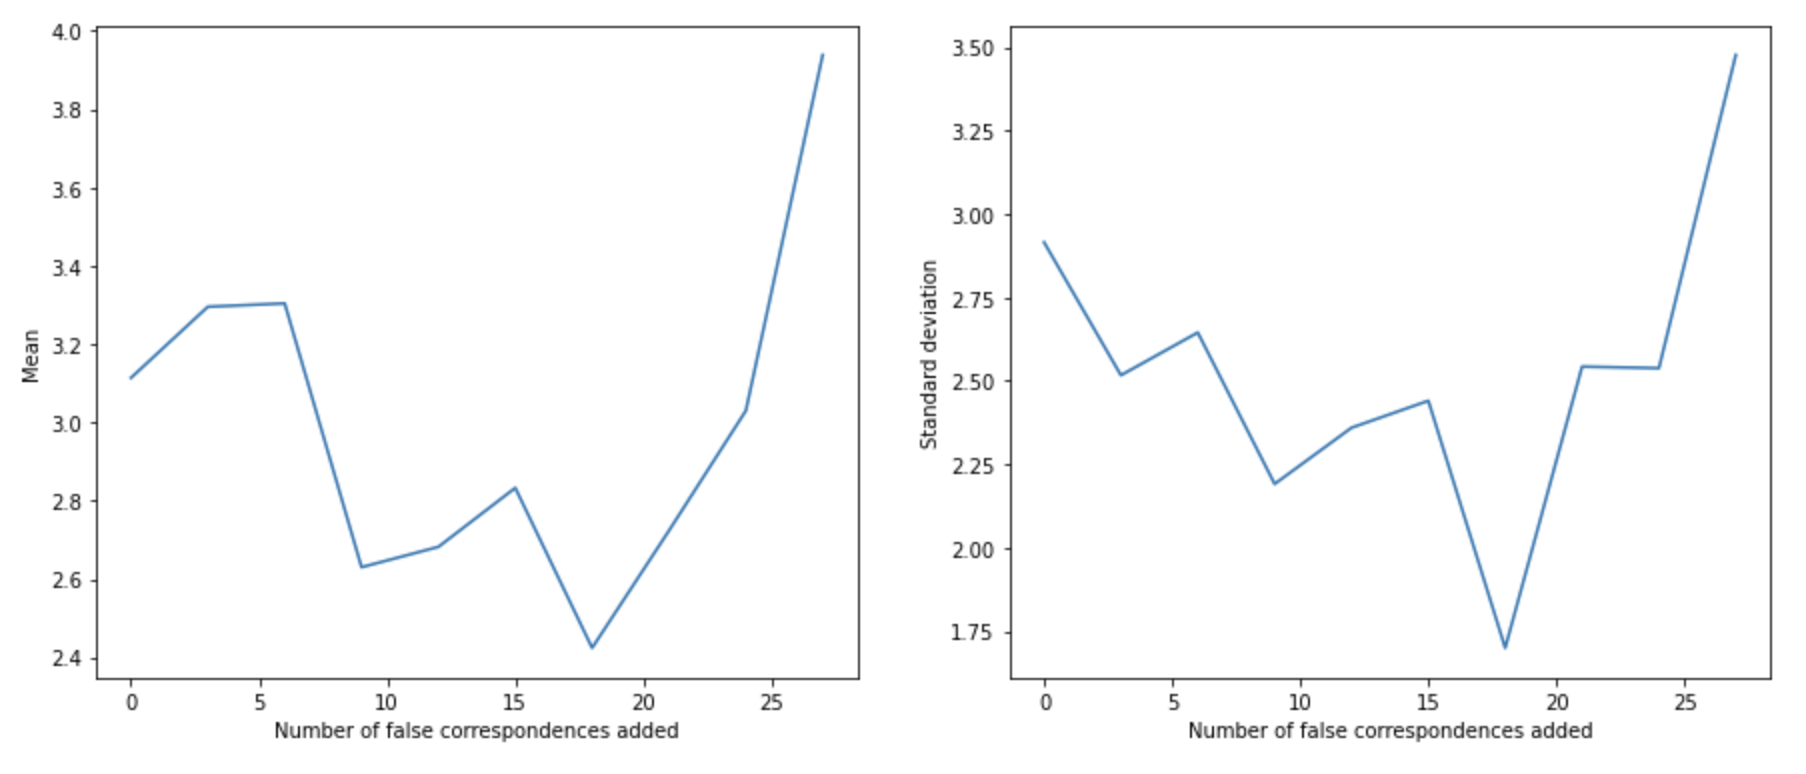
\includegraphics[width=\linewidth]{Materials/BaselineRansacMedian}
	\caption{The median mean and standard deviation after 10 Ransac runs with increasing number of false correspondences added to the manually found correspondences.}
	\label{BaselineRansacMedian}
\end{figure}
As seen the median mean and standard deviation only changes slightly, however, both show a tendency to grow quite rapidly when adding more than 18 false correspondences. This would equate to when the data consists of more than 42\% outliers Ransac begins to break down. This shows using Ransac makes the estimation of the fundamental matrix \textit{very} robust. We do however need to keep in mind that the false correspondences added here are random points in the two images, and so they with high probability false \textit{completely} out of line with our inliers. This might be a reason why we can include so many false correspondences.

\subsubsection{Scanline agreement using Ransac}
Taking a visual look at using Ransac, we can report the result of running Ransac on the 25 correspondences manually found, and from the inliers, estimate the fundamental matrix. This can be seen in \autoref{BaselineRansac}.
\begin{figure}[h]
	\centering
	\begin{subfigure}{0.48\linewidth}
		\centering
		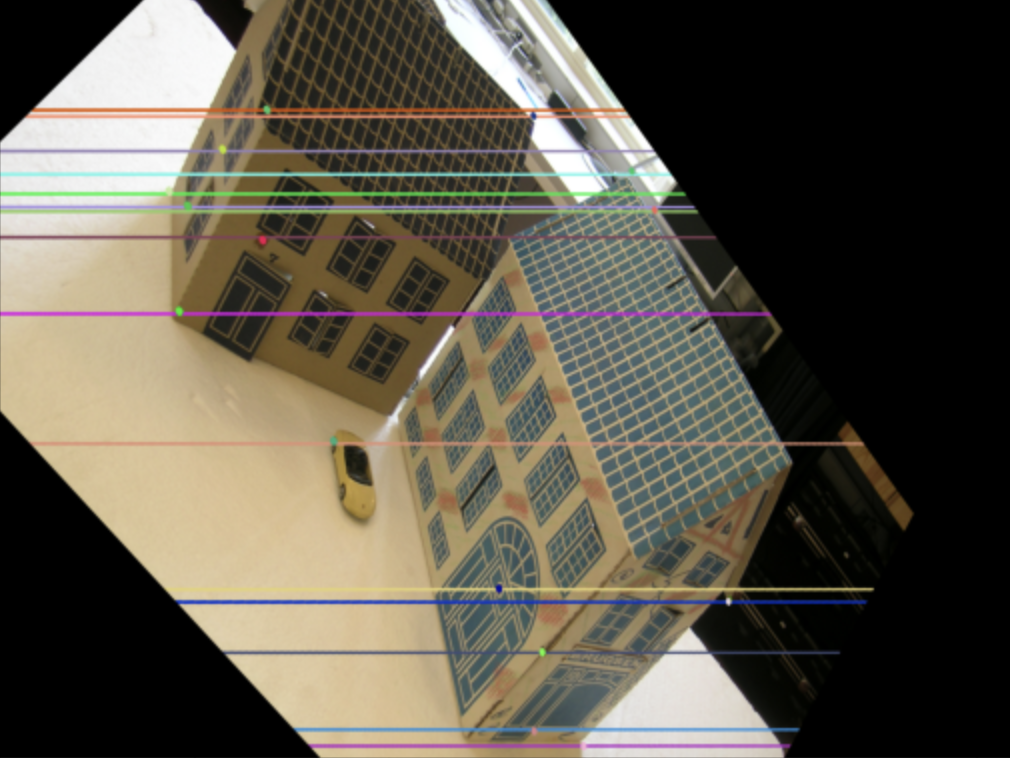
\includegraphics[width=\linewidth]{Materials/BaselineARansac}
	\end{subfigure}
	\begin{subfigure}{0.48\linewidth}
		\centering
		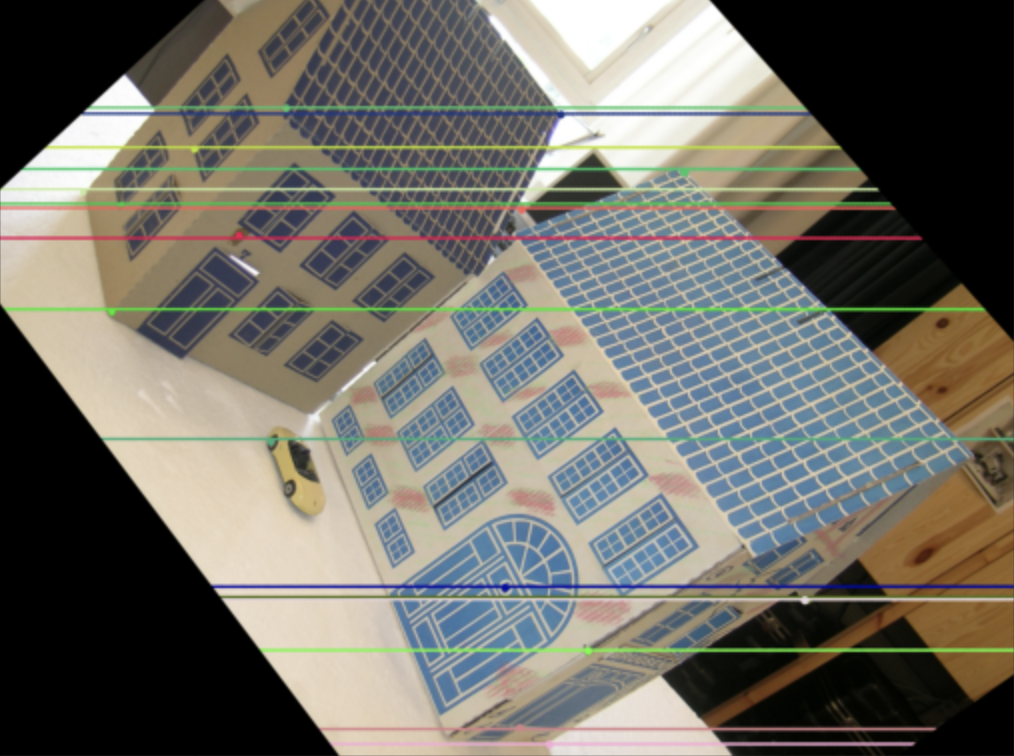
\includegraphics[width=\linewidth]{Materials/BaselineBRansac}
	\end{subfigure}
	\caption{Result of using Ransac on the original 25 correspondences before estimating the fundamental matrix and then bringing the images to scanline agreement.}
	\label{BaselineRansac}
\end{figure}
We here find a \textbf{mean} of \textbf{4.14} and a \textbf{standard deviation} of \textbf{2.57} of the scanline agreement error, which is a significant improvement over not using Ransac.